\chapter{Results and Observations}

\section{Normal Stack Setup}
Following the \texttt{jal} instruction into the \texttt{vulnerable} function, a 16-byte stack frame is allocated. The \texttt{sw ra, 12(sp)} instruction executes normally. In the register panel, \texttt{ra} (\texttt{x1}) holds the legitimate return value \texttt{0x00000004}. Correspondingly, the memory at \texttt{sp+12} is anchored precisely at \texttt{0x00000004}. At this point, the pipeline displays all five stages operating under normal IF/ID/EX/MEM/WB sequences.

\begin{figure}[h]
  \centering
  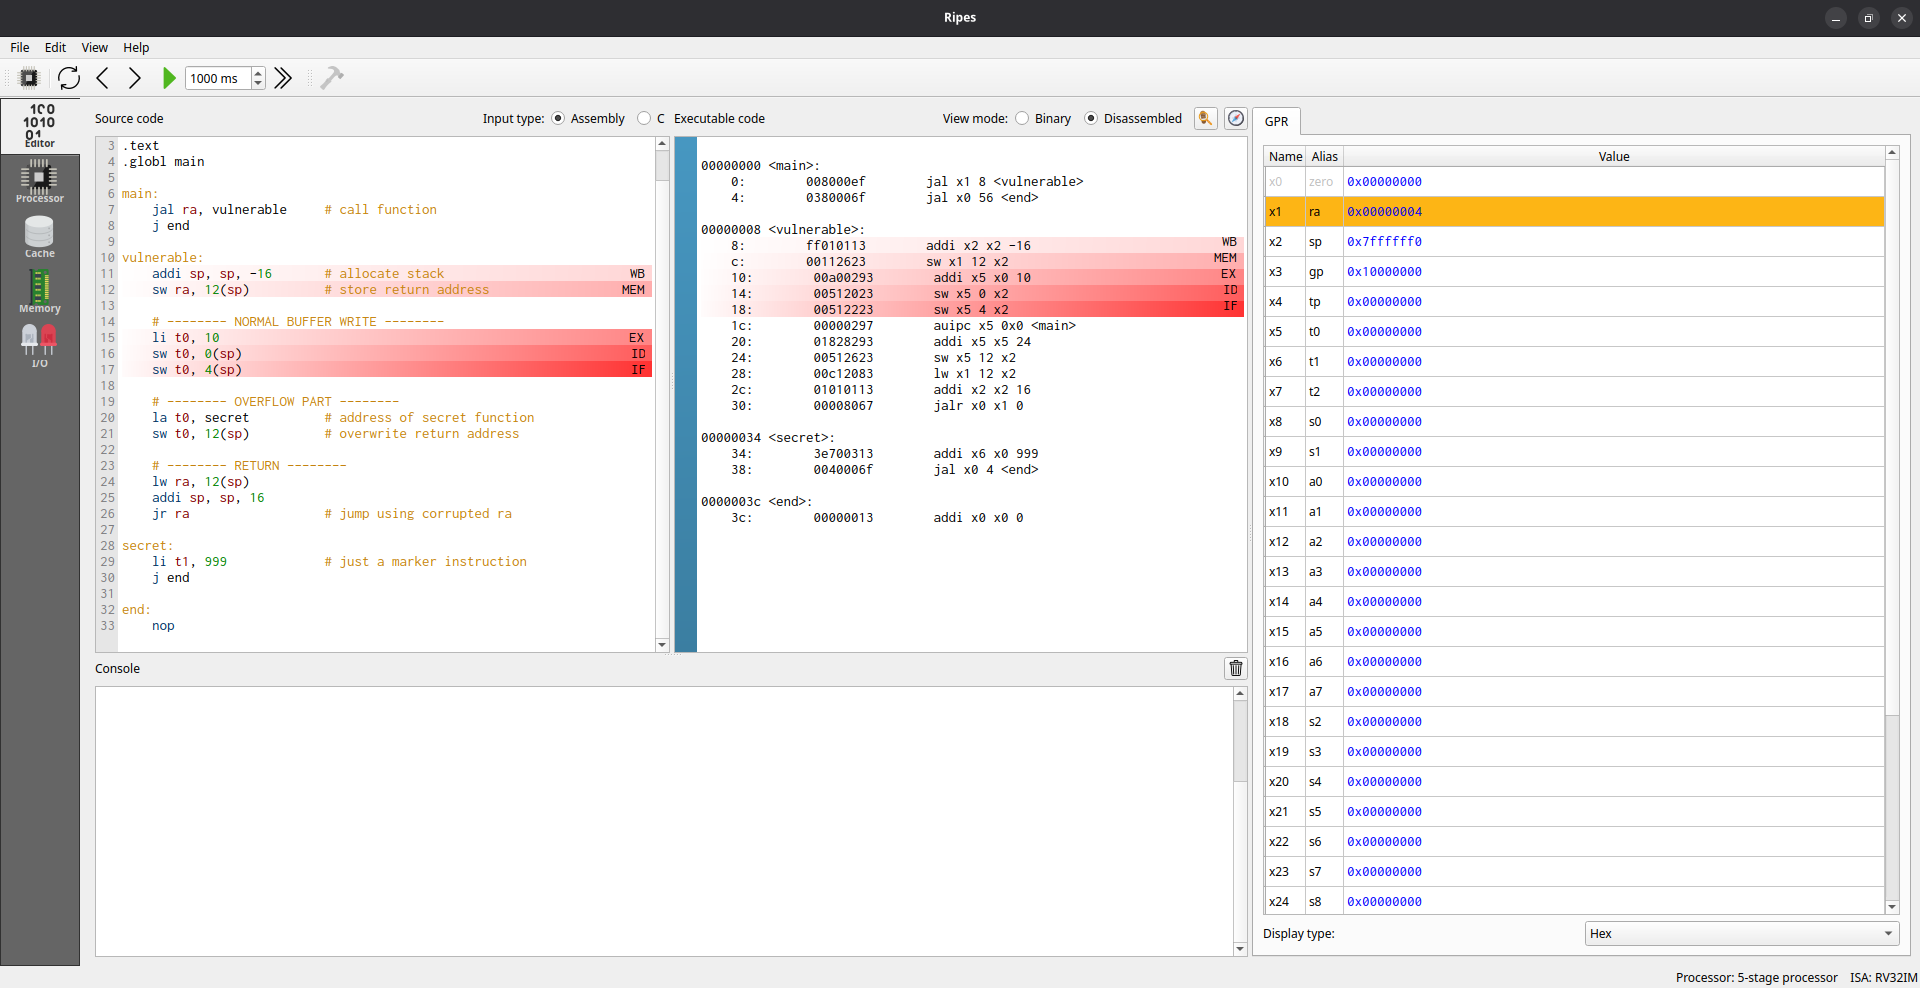
\includegraphics[width=0.8\textwidth]{images/ss2.png}
  \caption{Register file showing \texttt{ra=0x00000004} after legitimate save.}
  \label{fig:ss2}
\end{figure}

\section{Buffer Write Phase}
The standard buffer writes execute next: \texttt{sw t0, 0(sp)} and \texttt{sw t0, 4(sp)}. Memory observations confirm that \texttt{sp+0} and \texttt{sp+4} now contain \texttt{0x0000000A} (the value 10). Crucially, the target slot at \texttt{sp+12} remains intact with the value \texttt{0x00000004}.

\section{The Overflow Event}
The critical simulated breach occurs at the execution of \texttt{sw t0, 12(sp)}. The instruction proceeds to the MEM stage where it overwrites the architectural return slot. 

\begin{figure}[h]
  \centering
  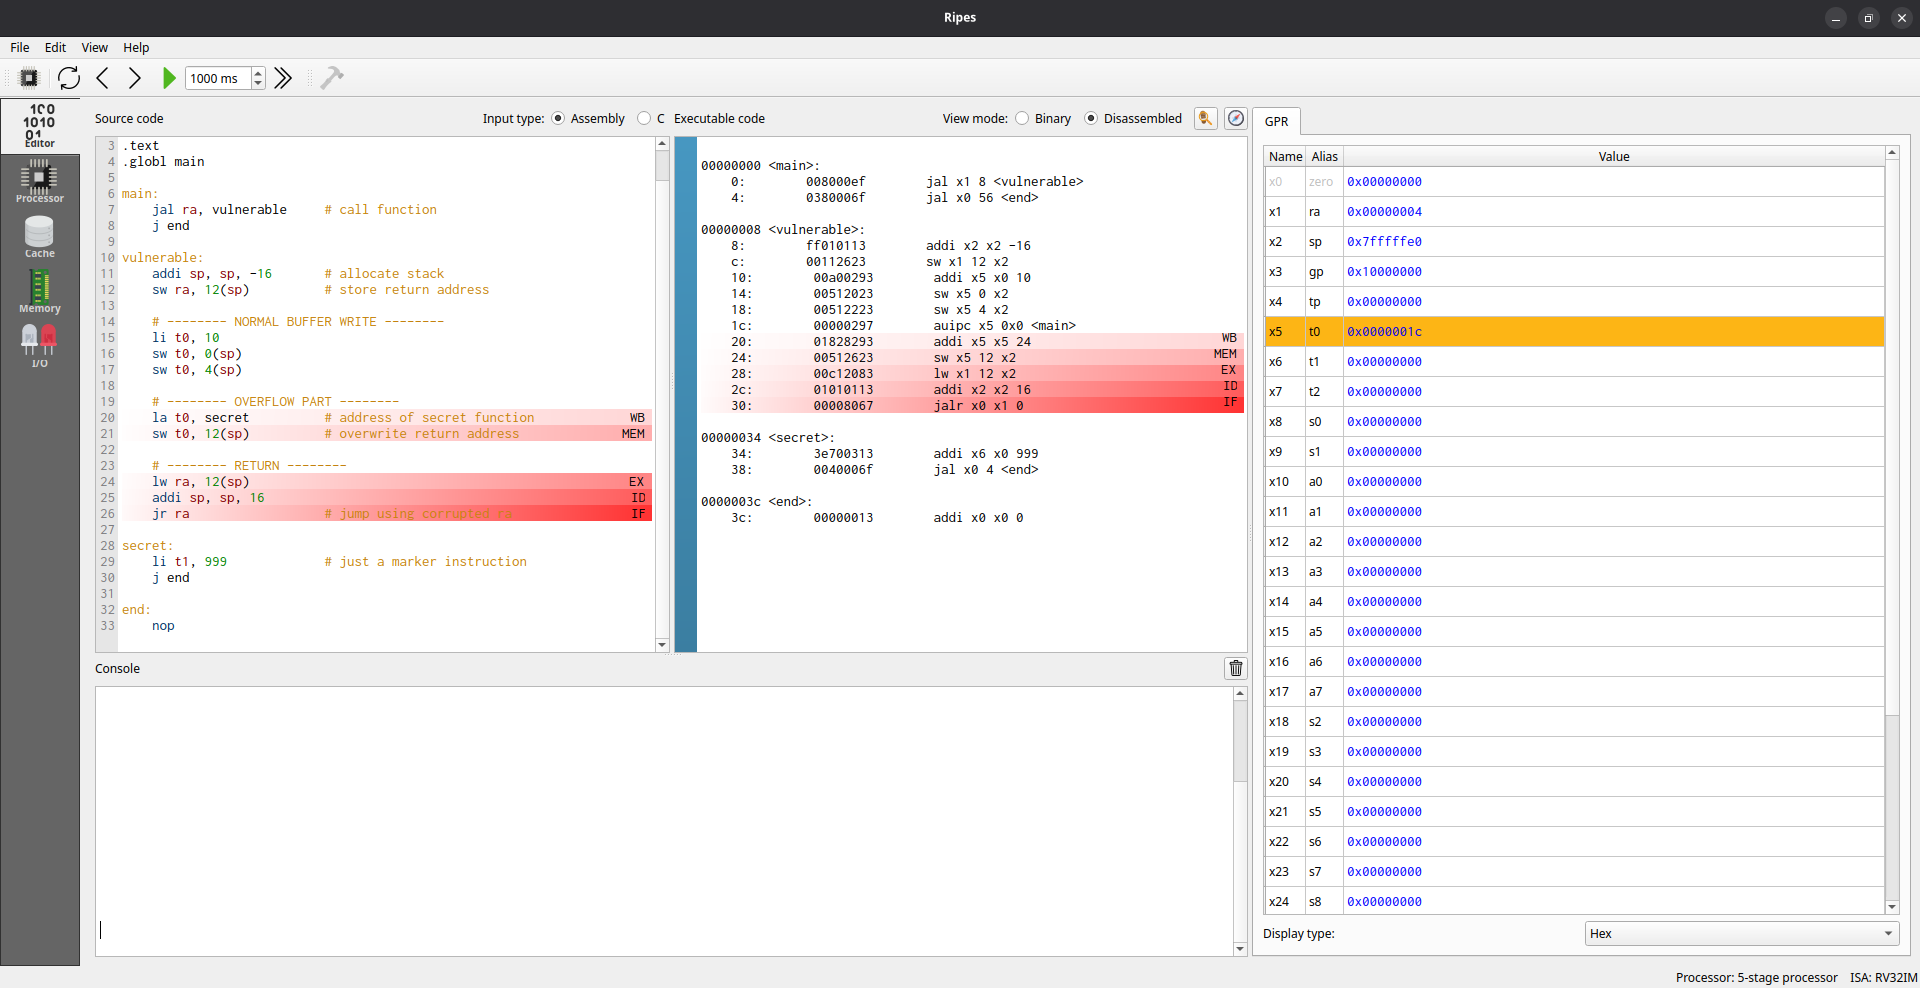
\includegraphics[width=0.8\textwidth]{images/ss3.png}
  \caption{\texttt{sw t0,12(sp)} in MEM stage --- overflow instruction executing.}
  \label{fig:ss3}
\end{figure}

Memory observation immediately highlights that \texttt{sp+12} has changed from \texttt{0x00000004} to \texttt{0x00000034} (the address of our \texttt{secret} function). This constitutes the core buffer overflow: a protected memory location is destructively overwritten.

\section{Return Address Corruption}
During the function epilogue, the \texttt{lw ra, 12(sp)} instruction restores the context. However, because memory was corrupted, the register file reads the overwritten value. The state of \texttt{ra} (\texttt{x1}) shifts from \texttt{0x00000004} to \texttt{0x00000034}. 

\begin{figure}[h]
  \centering
  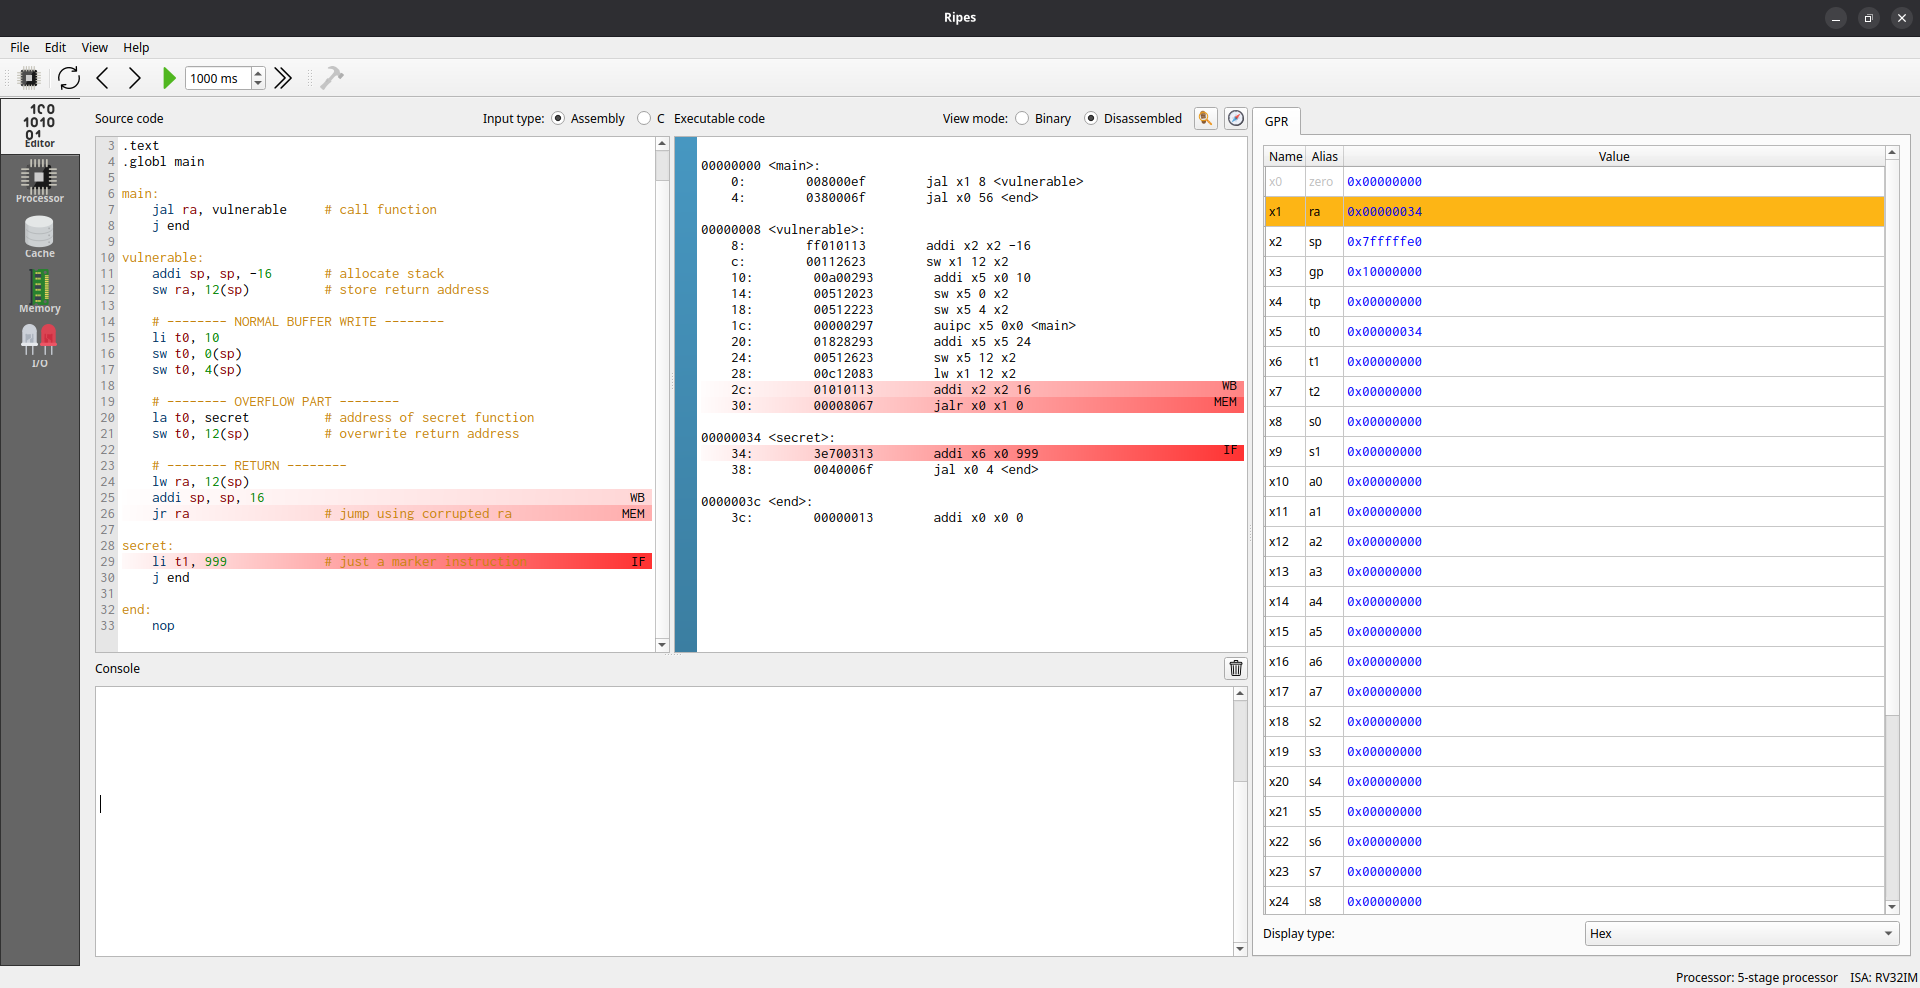
\includegraphics[width=0.8\textwidth]{images/ss4.png}
  \caption{\texttt{ra} corrupted to \texttt{0x00000034}; \texttt{li t1,999} is the current instruction.}
  \label{fig:ss4}
\end{figure}

\section{PC Hijack via \texttt{jr ra}}
The consequence of the corrupted return address manifests via the \texttt{jr ra} instruction. Instead of returning control to \texttt{main}, the Program Counter explicitly jumps to \texttt{0x00000034}. Execution of \texttt{li t1, 999} operates as empirical proof that code inside the \texttt{secret} function is currently executing. The normal intended path (\texttt{main} $\rightarrow$ \texttt{vulnerable} $\rightarrow$ \texttt{main}) is transformed into the hijacked path (\texttt{main} $\rightarrow$ \texttt{vulnerable} $\rightarrow$ \texttt{secret}).

\section{Control Hazard in the Pipeline}
Monitoring the Ripes pipeline diagram exposes a critical effect on dynamic scheduling. The \texttt{jr ra} instruction resolves in the EX stage. Due to the branch, speculative fetches—such as \texttt{li t1, 999} in ID, and \texttt{j end} in IF—are fed into the pipeline. This introduces a control hazard where the processor cannot determine the target natively until EX finishes. Consequently, a 2-cycle penalty is incurred as these instructions represent the inadvertently accepted path.

\begin{figure}[h]
  \centering
  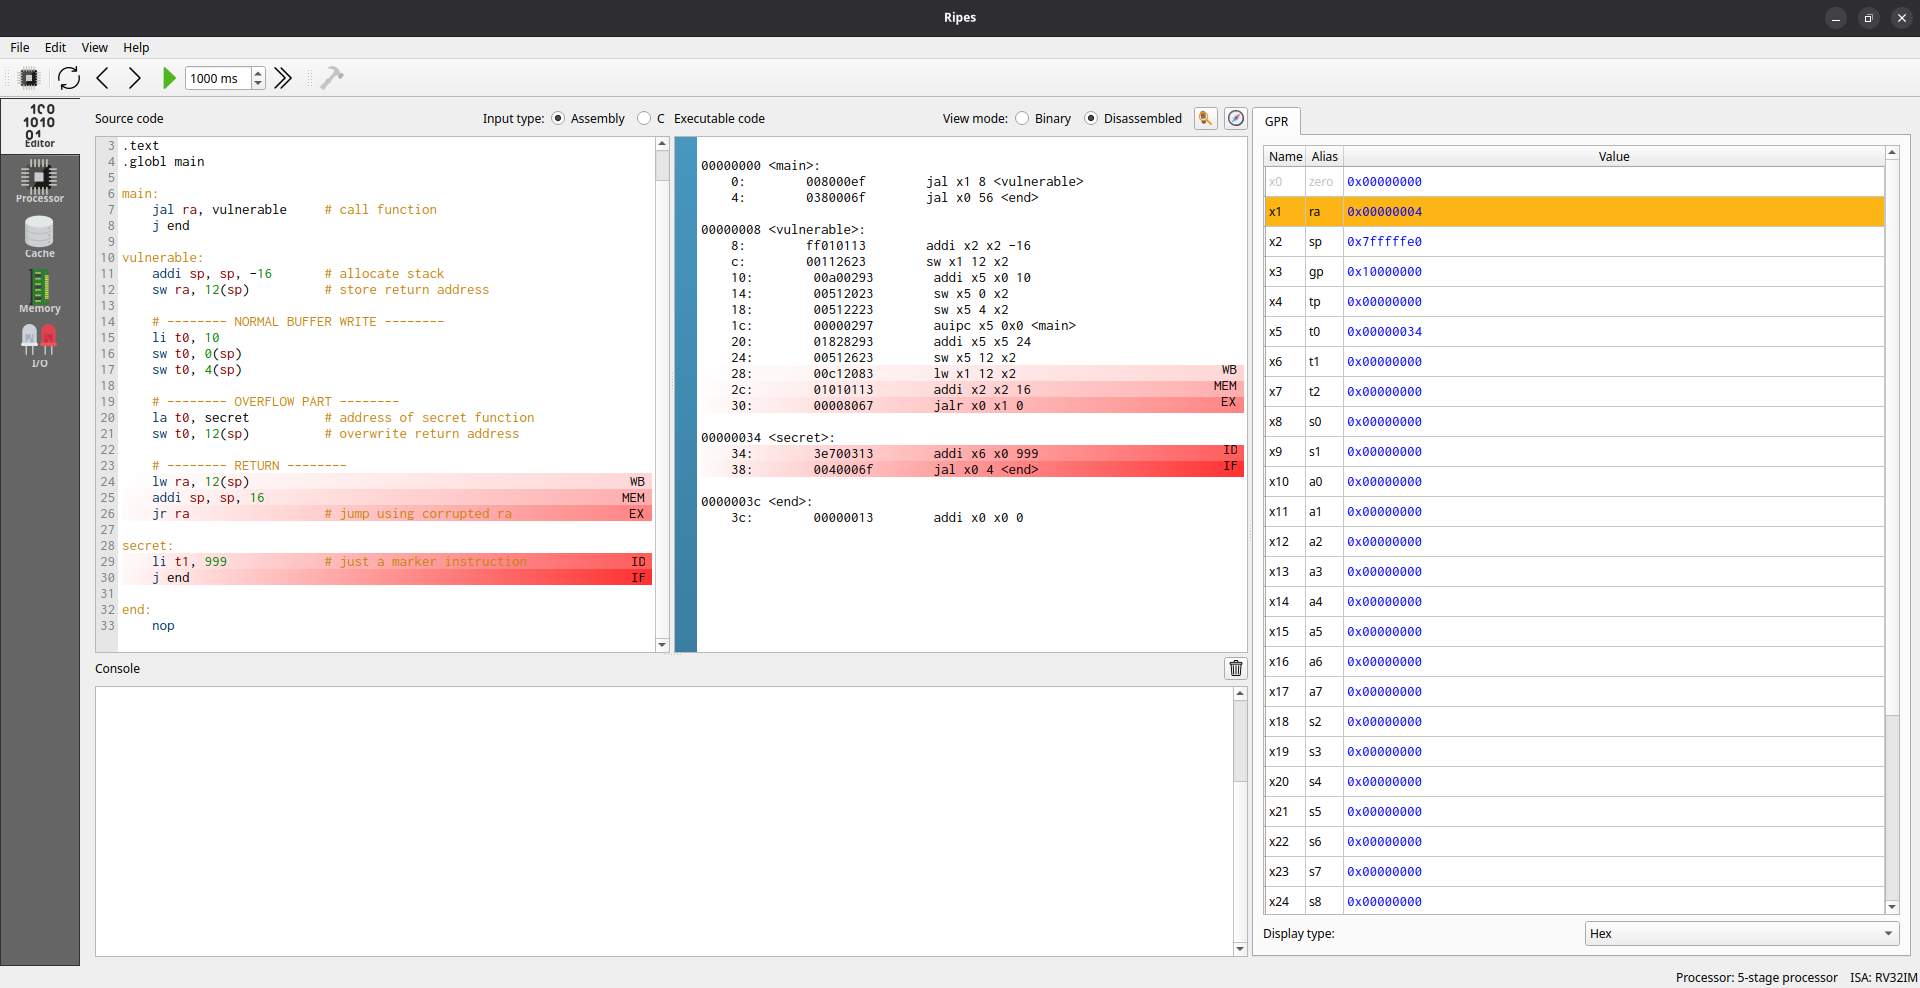
\includegraphics[width=0.8\textwidth]{images/ss5.png}
  \caption{\texttt{jr ra} in EX stage; \texttt{secret} instructions in ID and IF.}
  \label{fig:ss5}
\end{figure}

\section{Memory Comparison (Before vs After)}
The pre-condition and post-condition memory dumps reinforce the precision of the attack vector.

\begin{figure}[h]
  \centering
  \begin{minipage}{0.48\textwidth}
    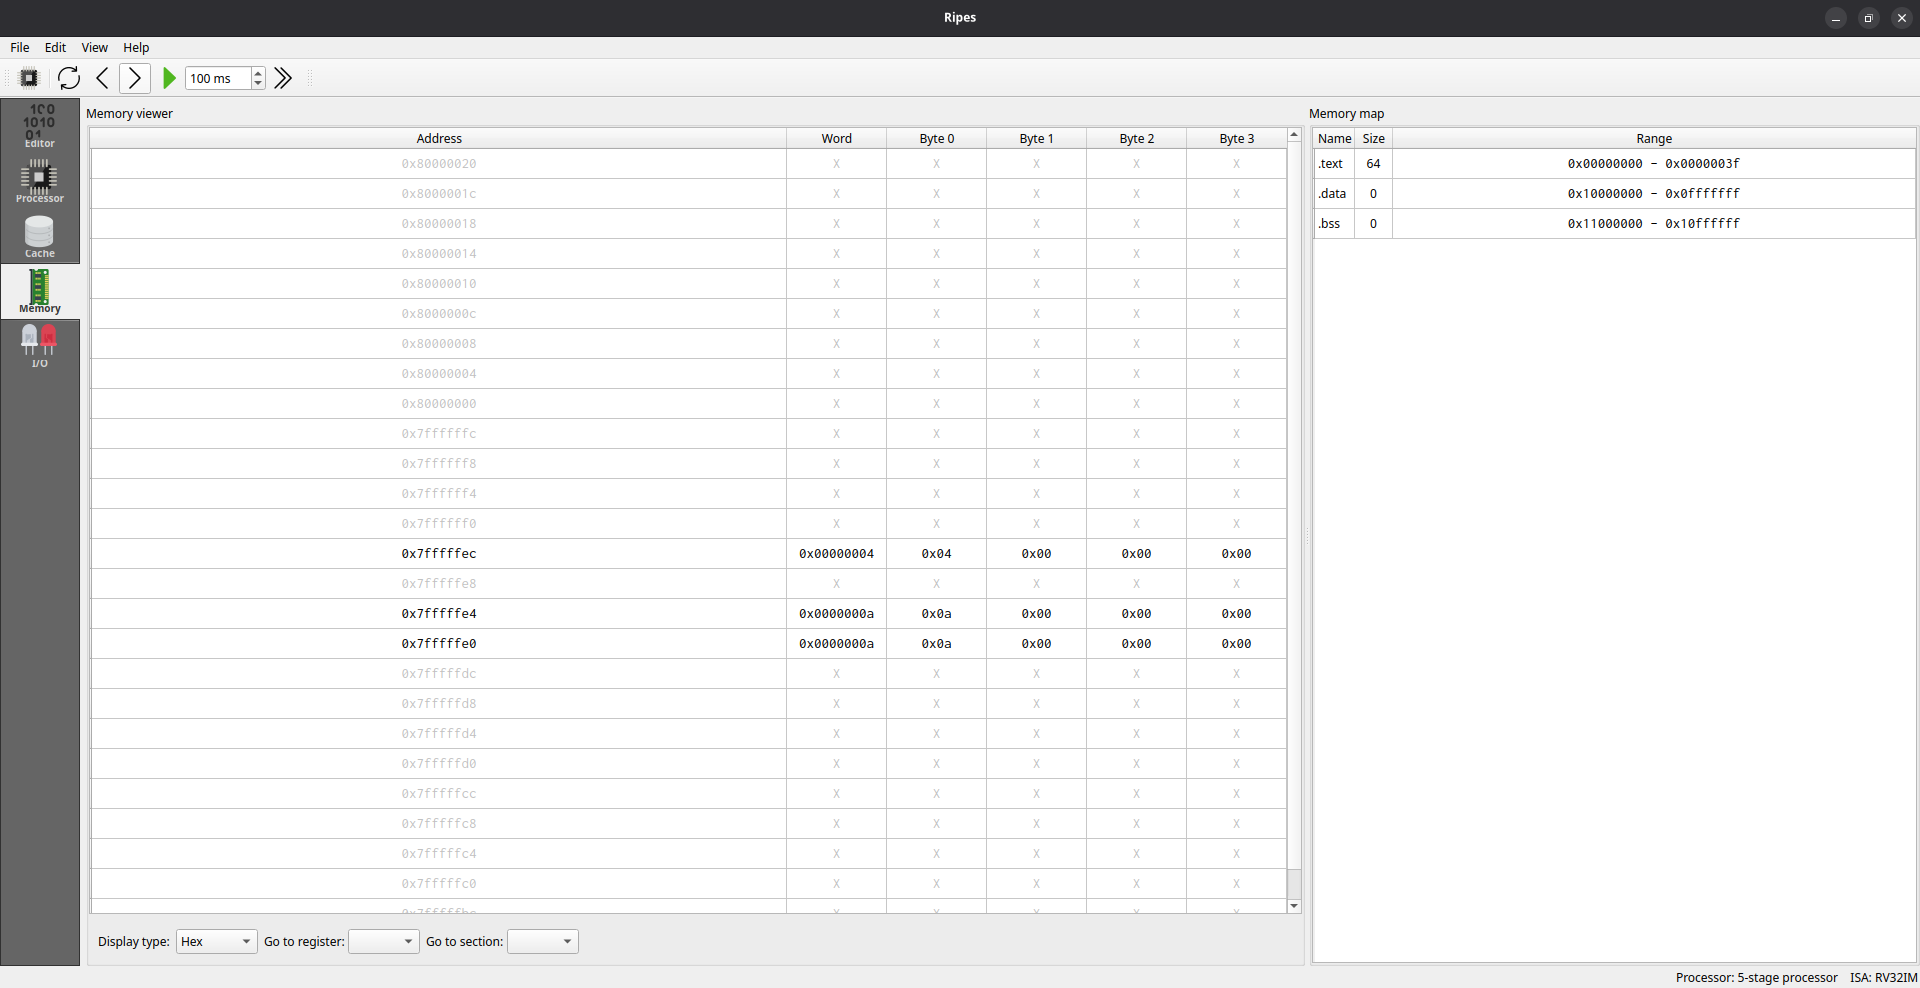
\includegraphics[width=\textwidth]{images/memory_before.png}
    \caption*{Before: \texttt{sp+12 = 0x00000004}}
  \end{minipage}
  \hfill
  \begin{minipage}{0.48\textwidth}
    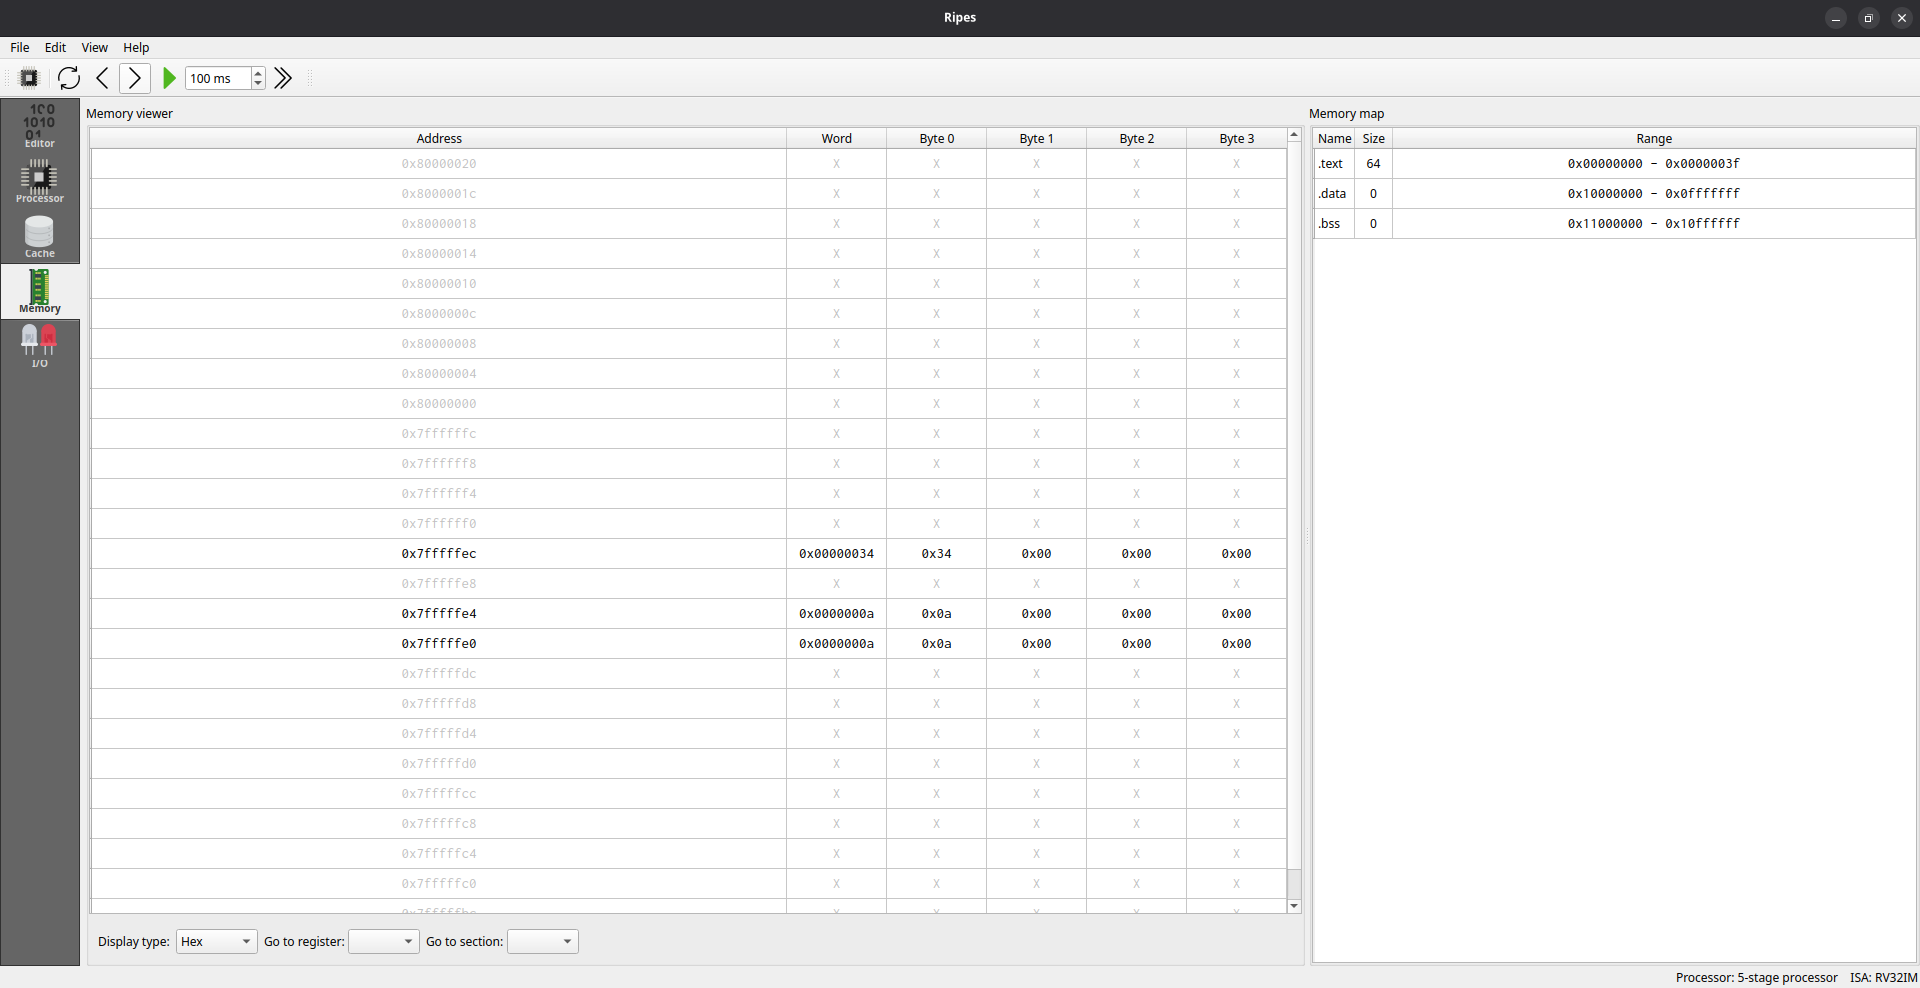
\includegraphics[width=\textwidth]{images/memory_after.png}
    \caption*{After: \texttt{sp+12 = 0x00000034}}
  \end{minipage}
  \caption{Side-by-side memory comparison showing return address corruption at sp+12.}
  \label{fig:memory_comparison}
\end{figure}

\section{Output Analysis Table}
The empirical mapping of execution states over the entirety of the attack chain is compiled below:

\begin{table}[h]
\caption{Output Analysis: Register and Memory State at Each Execution Stage}
\centering
\begin{tabular}{|c|l|l|l|}
\hline
\textbf{Stage} & \textbf{Condition} & \textbf{Register/Memory State} & \textbf{Behavior} \\
\hline
1 & Before Function Call & \texttt{ra} = return to \texttt{main} & Normal execution begins \\
2 & After \texttt{jal} & \texttt{ra} updated & Control to \texttt{vulnerable} \\
3 & Stack Setup & \texttt{sp} decreased, \texttt{ra} at \texttt{12(sp)} & Stack frame created \\
4 & Normal Buffer Write & \texttt{0(sp)}, \texttt{4(sp)} updated & Valid memory ops \\
5 & Before Overflow & \texttt{ra} in memory = original & System stable \\
6 & \textbf{After Overflow} & \textbf{\texttt{12(sp) = secret addr}} & \textbf{Return addr CORRUPTED} \\
7 & Load Return Address & \texttt{ra} = address of \texttt{secret} & Corrupted value loaded \\
8 & Function Return (\texttt{jr ra}) & \texttt{PC} = \texttt{secret} & Control flow changed \\
9 & Execution at \texttt{secret} & \texttt{t1 = 999} & Unexpected instruction \\
10 & Program End & Jump to \texttt{end} & Abnormal termination \\
\hline
\end{tabular}
\end{table}
